\documentclass[%
paper=a4,						% alle weiteren Papierformat einstellbar
%landscape,						% Querformat
fontsize=11pt,					% Schriftgröße (12pt, 11pt (Standard))
%BCOR1cm,						% Bindekorrektur, bspw. 1 cm
DIV=calc,						% führt die Satzspiegelberechnung neu aus
								% s. scrguide 2.4
%twoside,						% Doppelseiten
%twocolumn,						% zweispaltiger Satz
parskip=half,					% Absatzformatierung s. scrguide 3.1
%headsepline,					% Trennline zum Seitenkopf	
%footsepline,					% Trennline zum Seitenfuß
%titlepage,						% Titelei auf eigener Seite
headings=normal,				% Überschriften etwas kleiner (smallheadings)
%idxtotoc,						% Index im Inhaltsverzeichnis
%liststotoc,					% Abb.- und Tab.verzeichnis im Inhalt
bibliography=totoc,				% Literaturverzeichnis im Inhalt
%abstracton,					% Überschrift über der Zusammenfassungan	
%leqno,   						% Nummerierung von Gleichungen links
%fleqn,							% Ausgabe von Gleichungen linksbündig
%draft							% überlangen Zeilen in Ausgabe gekennzeichnet
]
{scrartcl}

\usepackage[pdftex]{graphicx} 
\usepackage[english]{babel}	
\usepackage[utf8]{inputenc}		
\usepackage[T1]{fontenc}								
\usepackage{lmodern}
\usepackage{color}

% Links im PDF
\usepackage{hyperref}
\definecolor{LinkColor}{rgb}{0,0,0.5}
\hypersetup{
	colorlinks=true,
	linkcolor=LinkColor,
	citecolor=LinkColor,
	filecolor=LinkColor,
	menucolor=LinkColor,
	urlcolor=LinkColor}
	
%Kopf u. Fußzeilen
\usepackage{scrpage2}
\pagestyle{scrheadings}
\clearscrheadfoot
%\chead{}
%\ofoot{}
\cfoot{\pagemark}

\usepackage{mdwlist}
\usepackage{csquotes}

% Neues bibliographie paket
% style=apa
\usepackage[isbn=false,url=false, doi=false, backend=biber, style=numeric]{biblatex}
\DeclareLanguageMapping{american}{american-apa}

\KOMAoptions{DIV=last}


\addbibresource{Forschungsmethoden-uebung-3.bib}

\title{Agile Software Development Methodologies}
\date{}
\author{Bernhard Fleck \and Rafael Konik \and Stephan Matiasch \and Harald Watzke}

\begin{document} 

\maketitle

\section*{Abstract} % (fold)
\label{abstract}

The process of software development is evolving all the time. There are many
different ways for companies to develop software, but most of them use the
heavyweight and lightweight approach. He heavyweight approach is considered as
the traditional way of software development, but in the last years the agile
approach came up. This approach uses short iterative development cycles. In
these cycles a small team develops a product, which is ready to release. There
are some different ways of agile software development. Two of them are Extreme
Programming (XP) and Scrum.

% section abstract (end)


\section{Introduction} % (fold)
\label{sec:introduction}

\zitat{The application of a systematic, disciplined, quantifiable approach to
the development, operation and maintenance of software.}~\cite{ieee90}

This is a very short but accurate definition of Software Engineering provided
by the \emph{IEEE Standard Glossary of Software Engineering Terminology}. The
most important part of this description is that it demands that the approach
of software development has to be quantifiable. Why is this so important?
Because the process of software development has to be understandable and also
measurable so that it can evolve.

Today the process of developing software has grown very extensive and involves
extensive planning, very detailed documentation and vast design. Many
companies have their own approach of developing software but usually companies
use the heavyweight and lightweight approach.  Heavyweight methodologies --
also considered as the traditional way of software development depend on
planning, documentation and design.  Over the past years another approach
gained popularity -- the lightweight approach -- also known as the agile
approach.

% section introduction (end)


\section{Agile Software Development} % (fold)
\label{sec:agile_software_development_methodologies}

The agile approach uses short term planning with iterative cycles and
does not directly involve long-term planning. Each cycle also has the
traditional phases such as requirement analysis, design, implementation and
testing but in a much smaller scale.

The team of typically 5--9 people works self-organizing and the members are
working in all functions (documentation, planning, coding, $\dots$) and the
communication is usually being held face-to-face or via user stories instead
of written documents. The user story is a quick and simple way of managing
customer requirements without the process of writing extensive documentation. The
user story is a small note card containing in a few sentences the requirements
a system must have.

At each end of a cycle the product is being shown to the stakeholders and
discussed with them for mutual satisfaction. The advantage of the agile
approach is that it is very flexible and minimizes the overall risks throughout
the developments process.

% section agile_software_development_methodologies (end)


\subsection{Extreme Programming (XP)} 

Extreme programming (XP) has evolved from the problems caused by long
development cycles of traditional development models~\cite{four}. It is used for
projects where requirements changes often during the project or for projects
where specific requirements are defined throughout the project. Originally
Extreme Programming was designed for team sizes from 3 to 12 people but due to
it's popularity it was also adapted for team sizes of 30 people. Though there
are problems with bigger teams because the main feature of Extreme Programming
is the direct cooperation between managers, clients and developers.~\cite{two}

The XP process can be characterized by short development cycles, incremental
planning, continuous feedback, reliance on communication, and evolutionary
design.~\cite{three}

The term \emph{extreme} comes from taking these commonsense principles and
practices to extreme levels. A summary of XP terms and practices is shown
below:~\cite{four}

\begin{description}

   \item[Planning] The programmer estimates the effort needed for
           implementation of customer stories and the customer decides the
           scope and timing of releases based on estimates. 
   \item[Small/short releases] An application is developed in a series of
           small, frequently updated versions. New versions are released
           anywhere from daily to monthly. 
   \item[Metaphor]
           The system is defined by a set of metaphors between the customer 
           and the programmers which describes how the system works. 
   \item[Simple Design] The emphasis is on designing the simplest possible solution that
is implemented and unnecessary complexity and extra code are removed immediately. 
   \item[Refactoring] It involves restructuring the system by removing duplication,
improving communication, simplifying and adding flexibility but without changing the functionality of the program.
   \item[Pair programming] All production code are written by two programmers on one
computer. 
   \item[Collective ownership] No single person owns or is responsible for individual code
segments rather anyone can change any part of the code at any time. 
   \item[Continuous Integration] A new piece of code is integrated with the current
system as soon as it is ready. When integrating, the system is built again and all tests must pass for the changes to be accepted. 
   \item[40-hour week] No one can work two overtime weeks in a row. A maximum of
40-hour working week otherwise it is treated as a problem. 
   \item[On-site customer] Customer must be available at all times with the development
team. 
   \item[Coding Standards] Coding rules exist and are followed by the programmers so
as to bring consistence and improve communication among the development team.~\cite{one}

\end{description}

\begin{figure}[h!]
   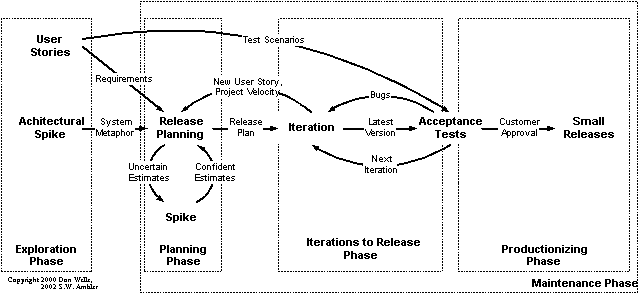
\includegraphics[width=1.0\columnwidth]{lifecycleXP}
   \caption{XP Lifecycle\protect\footnotemark}
\end{figure}

\footnotetext{\url{http://www.agilemodeling.com/essays/agileModelingXPLifecycle.htm}~(10.12.2012)} 

\subsection{Scrum}

The Certified Scrum Master program was published in 2002 by Ken Schwaber.

One Scrum team usually consists of 7 people, the Scrum Master, the Product
Owner and the developers. Those teams are self-directed work teams. In those
teams each member is able to manage all tasks and they all work together.

The most important finding is that small development teams with members who do
have all skills are working faster and more efficient. New achievements or new
knowledge is forwarded to the others at any time. Scrum uses a continuous
optimization progress and a one-piece-flow.~\cite{five}

\minisec{Roles in a Scrum team}

\begin{description}
   \item[Scrum Master] The Scrum Master is not part of the development team and
           he has to ensure that the Scrum project will succeed. He also has
           to ensure that nobody interferes in the organization of the team
           and that the team removes impediments.
   \item[Product Owner] The Product Owner decides the order of the user 
           stories, but does not decide how the product has to be made.
   \item[Development Team] The Development Team decides what it is capable of, 
           creates the product and has to ensure the quality of it. They work
           together to deliver the promised product.~\cite{five,eight}
\end{description}

\minisec{Important roles outside the Scrum team}

\begin{description}
   \item[The Manager] The Manager is the head of development and says how
           the product has to be developed.
   \item[The Customer] The Customer is the one who made the assignment.
   \item[The User] The User uses the product and gives feedback.~\cite{five}
\end{description}

Scrum is following the PDCA-Cycle (Plan-Do-Check-Act). In order of the
continuous optimization progress the project passes many Sprints. At the end
of each Sprint there is delivered usable software.

The one-piece-flow means that the development team is working exactly on one
functionality at the same time. Throughout this principle there is delivered
one functionality after the other. In each sprint the bugs are removed
immediately. If there comes up a new idea during a Sprint, it is put in the Product
Backlog and implemented in one of the next Sprints.

Another important principle is the Pull-Principle. It says that the
functionalities are implemented according to the requirements of the users.
The contrary principle would be the Push-Principle.~\cite{five}

\minisec{Artifacts}

\begin{description}
   \item[Product Backlog] The Product Backlog defines the prioritized user
           stories.
   \item[Sprint Backlog] The Sprint Backlog defines the goals the development
           team promised for the current Sprint.
   \item[Sprint Burndown Chart] The Sprint Burndown Chart contains the work
           remaining in the current Sprint.
   \item[Release Burndown Chart] The Release Burndown Chart contains the remaining
           user stories.~\cite{eight}
\end{description}

\minisec{One Sprint}

Each sprint should take at least one week and maximal four weeks. At the beginning
there are two Sprint Meetings. In the first Sprint Meeting the Product Owner
presents the Product Backlog to the team. In this Product Backlog he
prioritized the user stories. The Product Owner also makes arrangements with
the team about the criteria that the product should fulfill at the end of the
Sprint. At the end the development team has to tell the Scrum Master how many
user stories it promises to fulfill during the next Sprint.

In the second Meeting the development team discusses the \emph{How} of the
promised user stories. After this meeting there usually is a Sprint Backlog,
which illustrates the tasks of the following Sprint.

On each day there is Daily Scrum Meeting. During this meeting the team members
exchange information about the project.

After one sprint there is a Sprint Review. The development team reveals the
product to the Product Owner, who compares it with the Product Backlog and
decides if the Goal for this Sprint has been achieved. Afterwards the Users
are able to actually use the product and give feedback.  At the end of each
Sprint the functionality has to work and has to be able to be delivered to the
User.

Between the review and the next Sprint Planning Meeting there is the
Retrospective. During this part of the project the team should take advantages
of the experiences they made throughout the project and should look for
improvements. The Manager, the Customer and the User are not allowed to commit
these Retrospective Meetings except they are invited.~\cite{five,seven,eight}

\begin{figure}[h!]
   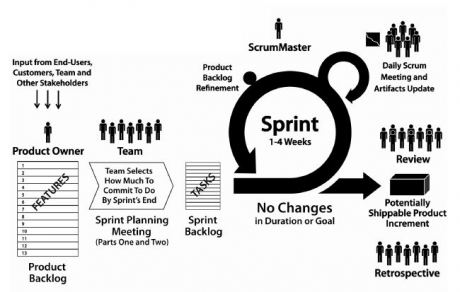
\includegraphics[width=1.0\columnwidth]{scrum-methodology}
   \caption{Scrum Lifecycle\protect\footnotemark}
\end{figure}

\footnotetext{\url{https://www.realmdigital.co.za/post/whats-scrum-and-how-do-we-use-it}~(11.12.2012)}

\section{Conclusion} % (fold)
\label{sec:conclusion}

Agile development is not defined by a small set of practices and techniques.
From the set of success stories and anecdotal evidence we have come to believe
that agile development defines a strategic capability, a capability to create
and respond to change, a capability to balance flexibility and structure, a
capability to draw creativity and innovation out of a development team, and a
capability to lead organizations through turbulence and uncertainty~\cite{one}. Modern
companies want to respond quickly to customer wishes and they need to focus on
delivering innovative product and adapt to market conditions.

Agile Software Development is very dominant now and surely will be in the
future too. Modern Software development project can benefit from the agile
methodologies and others can benefit more from the traditional methodologies.
We can tell for sure that every software development project is different and,
although it's good to have some approaches that we can lean on, one thing is
clear: \emph{There is no best way to catch a mouse.}

% section conclusion (end)

%\nocite{*}
\printbibliography

\end{document}
